\documentclass[a4paper,12pt]{article}
\usepackage{mathtools,amsfonts,amssymb,amsmath, bm,commath,multicol}
\usepackage{algorithmicx, tkz-graph, algorithm, fancyhdr, pgfplots}
\usepackage{fancyvrb, amsthm, csquotes, booktabs}
\usepackage[backend=biber, citestyle=authoryear]{biblatex}
\addbibresource{thesis.bib}

\usepackage[noend]{algpseudocode}

\newtheorem{theorem}{Theorem}[section]
\newtheorem{proposition}{Proposition}[theorem]
\newtheorem{lemma}[theorem]{Lemma}
\DeclareMathOperator*{\argmin}{argmin}

\newcommand{\diagmat}[1]{\left[%
\begin{array}{@{}c@{}c@{}c@{}}
\diagdown &    & \\
          & #1 & \\
          &    & \diagdown
\end{array}\right]
}

\pagestyle{fancy}
\fancyhf{}
\rhead{Nandan Rao}
\lhead{Mapping Between Personality Factor Spaces}
\rfoot{\thepage}

\begin{document}

\title{Mapping Between Personality Factor Spaces}

\author{Nandan Rao}

\maketitle

\begin{abstract}
  We use techniques taken from, and some further inspired by, original research in personality traits to examine the personality survey data from 94 students in 2 classes in 2 schools in Barcelona. We find that the Big Five personality traits are definitively...
\end{abstract}

\section{Background}
It's easy to measure the knowledge a student has memorized: sit them down, watch them to make sure they have not written any notes on their hands, and make them answer questions. If they don't remember the facts you ask them, they will answer incorrectly.

In this way we have measured the knowledge of students for many years, and through this we have assessed the performance of our schools and education systems. Recently there has been a move to emphasize the importance of teaching and fostering noncognitive skills in our students however the task of measuring these skills is still an unsolved problem.

A long standing and oft-proved theory in the literature of personality psychology is that there are five major axes, or factors, on which one can accurately describe the majority of differences in individuals noncognitive features, referred to as the Big Five personality traits. We will explore the history and repeat the methodologies of the original discoverers of this theory, but for now it suffices to say that this is, for our purposes, the psychological ground truth our work revolves around.

The Big Five personality traits were originally discovered, and continue to be measured, via survey questions. If your personality was to be measured, you might be given a survey in which you answer questions about yourself, after which the answers will immediately be translated into personality traits. Alternatively, the survey might be given to your peers, who answer similar questions regarding your personality, after which the answers are gathered and aggregated to calculate your personality score.

Clearly, surveys are problematic in the setting of school assessments. Students have no natural incentive to answer honestly, admitting to negative aspects of their personality, but many incentives can exist in the contrary. Clearly, peer-reviewing is no better in this regards. What is left then is to build accurate predictors of these personality traits with measures that cannot be gamed by the students or teachers.

When one is tasked to find accurate predictors, it is natural to think of the task as one of prediction, gather labelled data, and use every technique one has in their supervised-learning toolbox to build an accurate model. To some degree we will be doing that, and a large part of this ongoing work involves the creation of that data. As of now, however, and most likely for the foreseeable future, the number of observations in this labelled data is extremely small. With a small number of observations, we are drastically restricted in our ability to build an accurate model with strong guarantees on out-of-sample accuracy.

The only savior we have in lieu of data is, as always, Theory. This thesis is a small step in thin this larger work, the primary goal here being simply to explore the theory behind these personality traits and validate this theory with the data we have. The secondary goal is to motivate the next steps in this research based on this core theory, our data, and a renewed understanding of our goals.

\section{History}

For a concise history of the lexical origins and process of discovery of the Big Five traits, we refer the reader to \cite{john1999}.

For our purposes, we start with \cite{norman1963}, who uses almost identical data collection and scoring techniques as the earlier \cite{tupes1961}, which, it should be noted, was the true first Big Five discovery. But where the previous study relied on visual rotation techniques for orthogonal rotation procedures, only having access to an IBM 650 for one of their studies, \cite{norman1963} revisits the same ideas with fully modern techniques, using a computer for each and every rotation. Seeing as we, too, will use a computer for each and every rotation, and that Norman finds results almost identical to those from \cite{tupes1961}, this seems like a fair place to start.

This particular data set consists of four samples of male college students, each sample divided into small groups based on the dormitories or ROTC (military) training groups of the individuals. Each person was asked to rate peers from their group on a number of scales, which were taken as a subset of the results of \cite{tupes1958}.

It is worth noting a couple of interesting and pertinent observations one makes when reading Norman's work. The first is that the raters were required to rate one third of their peers being on one ``pole'' of each scale, one third on the other pole, and one third ``nuetral'', or unrated. For example, given the scale of ``Talkative-Silent'', the raters had to rate exactly one third of their peers as Talkative and one third as Silent. By Construction this creates mean-zero, symmetric ratings.

The second, related, fact we will note, is the way in which he notes the following:

\begin{displayquote}
By no means is there any indication of a large general factor, for instance, one attributable to general evaluative tendencies or social desirability, present anywhere in these results... It is thus reassuring to this writer at least, to observe that no factor was found which even closely resembled such a general evaluative response set effect in any of these analyses.
\end{displayquote}

We return to these notes when examining and considering possible problems in our own data. The technical factor analysis he employs is straightforward, and we will expound each term in the following section for those not already familiar. In few words, however: principle axes are found, after which varimax rotation is applied to achieve simple structure. He then examines these results and finds that the factors group the questions into the same groups as found in earlier studies, concluding that these factors are therefore consistent.

To compare factors between studies, Norman refers to the technique laid out in \cite{kaiser1971}.

\section{Models and Methodologies}

\newcommand{\X}{$\mathbf{X} \ $}
\newcommand{\F}{$\mathbf{F} \ $}
\newcommand{\Load}{$\mathbf{L} \ $}
\newcommand{\B}{\mathbf}

\subsection{An Orthogonal Factor Model}

We begin with the basic definition of an orthogonal factor model, along with covering the basic assumptions.
%
\begin{equation}
\mathbf{X} = \mathbf{F}\mathbf{L'} + \mathbf{E}
\end{equation}
%
Here we note that \X is a the traditional feature matrix, with mean zero, dimension (N,P). \F is the (N,M) matrix of ``factors'', the latent variables that represent our data in its true $M$-dimensional form ($M < P$). \Load  is the (M,P) ``loading'' matrix, also called the dictionary in signal processing or the components in PCA/SVD terminology, these are the coordinate axes of the subspace spanned by our currently orthogonal features within the original feature space. $\mathbf{E}$ is an error matrix. Note that this model assumes, clearly, that relationship between the latent ``factor'' variables and that of the observed variables is strictly linear.

We put the following restrictions on the terms:
%
$$
\mathbf{cov}(\mathbf{F}) = \mathbf{I}
$$
%
This is the basic assumption on orthogonality of the factors that allows this model to have a unique solution.
$$
\mathbf{cov}(\mathbf{E}) = \mathbf{\Psi} = \diagmat{\mathbf{\Psi}}
$$
%
We allow the errors of the factors to have individual variance, but the must be uncorrelated with each other. Note, that the case of $\mathbf{E} \sim N(0, \mathbf{I})$ is the assumption which turns this general orthogonal factor model into Principle Component Analysis. Avoiding that assumption and preferring a generative model allows us to learn both the factor values and variances through probabilistic likelihood. This is easily considered as a generative model, with an efficient EM algorithm solution available if the errors are assumed $\mathbf{E} \sim N(0, \mathbf{\Psi})$, where closed form solutions exist for the Gaussian likelihood at every step.

Restricting our errors to a world of Gaussianity also allows us to estimate the ``factor scores'', our $\B{F}$, via weighted least squares:

\begin{align*}
\mathbf{F}\mathbf{L'} + \mathbf{E} &= \mathbf{X} \\
\B{\hat{F}}\B{L'}\B{\Psi}^{-1}\B{L} &= \B{X}\B{\Psi}^{-1}\B{L}  \\
\B{\hat{F}} &= \B{X}\B{\Psi}^{-1}\B{L}(\B{L'}\B{\Psi}^{-1}\B{L})^{-1}
\end{align*}
%
Here it is clear to see that in the PCA case, with $\B{\Psi} = \B{I}$ and $\B{L}$ is orthogonal, this reduces to a simple dot product with the components:

$$
\B{\hat{F}} = \B{X}\B{L}
$$
%
\subsection{Orthogonal Rotation}
%
We refrain on giving a full exposition on rotation in factor models, directing the reader to \cite{}. It suffices our purposes to state a few simple mathematical facts that are not found everywhere but pertinent to our analysis here. Before that, however, we would simply clarify that the orthogonal factor model estimated above is unique only up to a orthogonal rotation of the loadings matrix. That is to say that the subspace of the factors within the original feature space is determined, but the coordinate axis can be orthogonally rotated and maintain the same covariance matrix estimation from the model.

This rotational ability is core to factor analysis, and will be core to our examination of the data. It will be useful to prove that, in the above factor model, a rotation matrix applied to the loadings will lead to estimation of factor scores rotated by the same matrix:

\begin{align*}
\B{\hat{F}T(LT)'\Psi^{-1}LT} &= \B{X\Psi^{-1}LT} \\
\B{\hat{F}TT'L\Psi^{-1}LTT'} &= \B{X\Psi^{-1}LTT'} \\
\B{\hat{F}L\Psi^{-1}L} &= \B{X\Psi^{-1}L}
\end{align*}
%
Where $\B{TT'} = \B{T'T} = \B{I}$ for any orthogonal rotation matrix.

\subsection{Simple Structure and Varimax}

Simple structure is a name given by Thurston in the oldest days of factor analysis, and refers to a loading matrix that loads each factor onto different variables and each variable onto only one factor, or definitely less than all, of the factors. The core idea is of course interpretability, but it goes further than that, with Thurston believing that factors based on a simple strucutre are side to the subspaces, rather than the variables themselves, and that these subspaces are likely to be consistent across different variables that are expressions of the same factors. While interesting, for our case, we examine it for the sake of interpretability.

Varimax is a technique that orthogonally rotates a matrix, in our case a loading matrix, in order to maximize a straightforward mathematical measure of such simple structure, namely: maximize the variance of the squared loadings across each factor. The measure, the normal varimax criterion, is presented below:

\begin{equation}
\frac{1}{P} \sum_{j=1}^M \bigg( \sum_{i=1}^P\Lambda_{ij}^4 - \bigg( \sum_{i=1}^P\frac{1}{P}\Lambda_{ij}^2\bigg)\bigg)
\end{equation}
%
Where $\Lambda$ refers to the normalized loadings. This objective will be most useful to us.

\section{Data}

The data used in this exploration is fairly simple, but it is also important to understand the greater data context in which this study is taking place.

Here we will analyze two groups of self-reported surveys, referred hereafter as Big Five and Others. These surveys were administered to students in two different classes, in different schools, with different teaching techniques. There are 94 students in total that answered these surveys. The Big Five survey is a questionnaire that has been created explicitly to measure the Big Five personality questions, and it comes with a ``key'', which explains which trait each question maps to. Each question maps positively to one trait only. The Others surveys consist of questions whose key has been intentionally hidden from the writer, but they purport to summarize a persons personality by the way in which they answer the questions in a similar fashion.

Outside of the scope of this paper, but in the scope of this work, is one other primary data set for which we currently have data: EEG data measured during Stroop, 3-back, and 2-back concentration tasks. Everything we do here is to be understood in the context of better understanding all aspects and requirements for techniques that can be used on this particular data set, which is decidedly very different in many ways, but which also purports to measure personality traits of individuals.

Furthermore, there are other opportunities to gather additional tests and measurements of these students, including how they cooperate under difficult conditions, tests for Mindset, and questions regarding social networks connections within the class. This data is not available to us at the moment, but should give a flavor for the variety over which our eventual prediction task will be expected to operate.

\begin{enumerate}
\item Experiments and challenges in which students cooporation
\end{enumerate}

\section{Theory + Data}

Here we seek to answer the fundamental question of this thesis: does the Big Five factor model describe the personalities recorded in our surveys? We will address this in the following ways:

\begin{enumerate}

\item Are the Big Five personality traits clearly present as factors in our Big Five survey?

\item How much variance in our Big Five survey does the official Big Five encoding explain, compared to our estimated factors, out of the variance in our data itself?

\item How do the latent factor representations of our two survey groups correlate?
\end{enumerate}

As set out in the beginning, the spirit of this journey is to understand the origins of these personality traits, and then to see if we find them in our own data. Norman's method primarily consisted of finding a principle axes solution and rotating the factors via varimax rotation. So we start with repeating exactly that process for our Big Five survey data, examining how much variance is explained, refer to table \ref{table:pca-variance}. We see that our first principle axes explain approximately 46\% of the variance of our data, while the same data, when interpreted via the official encoding for the Big Five traits, is explained only up to 37\%.

As discussed previously, PCA will differ from a maximum likelihood solution when the error variance is heterogeneous across factors. Given that we have reason to expect this possibility in our data, we estimate a generative model via expectation maximization and regenerate a similar table, table \ref{table:ml-variance}, where we see that now the percentage of explained variance by our factors has now been reduced to 42\%. Here we have an initial answer to question number 2.



\begin{table}
\begin{tabular}{lrrrrr}
\toprule
{} &          0 &         1 &          2 &         3 &         4 \\
\midrule
Components &  23.543123 &  7.580135 &   6.321525 &  5.111549 &  3.795437 \\
Varimax    &  14.691594 &  5.573418 &  12.284804 &  7.432257 &  6.369697 \\
Big Five   &   7.569611 &  7.590264 &   7.664056 &  6.073631 &  8.321417 \\
\bottomrule
\end{tabular}
\caption{Explained Variance of PCA}\label{table:pca-variance}
\end{table}


\begin{table}
\begin{tabular}{lrrrrr}
\toprule
{} &          0 &          1 &         2 &         3 &         4 \\
\midrule
Components &  22.586949 &   6.474895 &  5.544954 &  4.367940 &  2.922496 \\
Varimax    &  13.645560 &  10.342161 &  7.858926 &  4.543434 &  5.507152 \\
Big Five   &   7.569611 &   7.590264 &  7.664056 &  6.073631 &  8.321417 \\
\bottomrule
\end{tabular}
\caption{Explained Variance of Maximum Likelihood Estimation}\label{table:ml-variance}
\end{table}

\begin{figure}
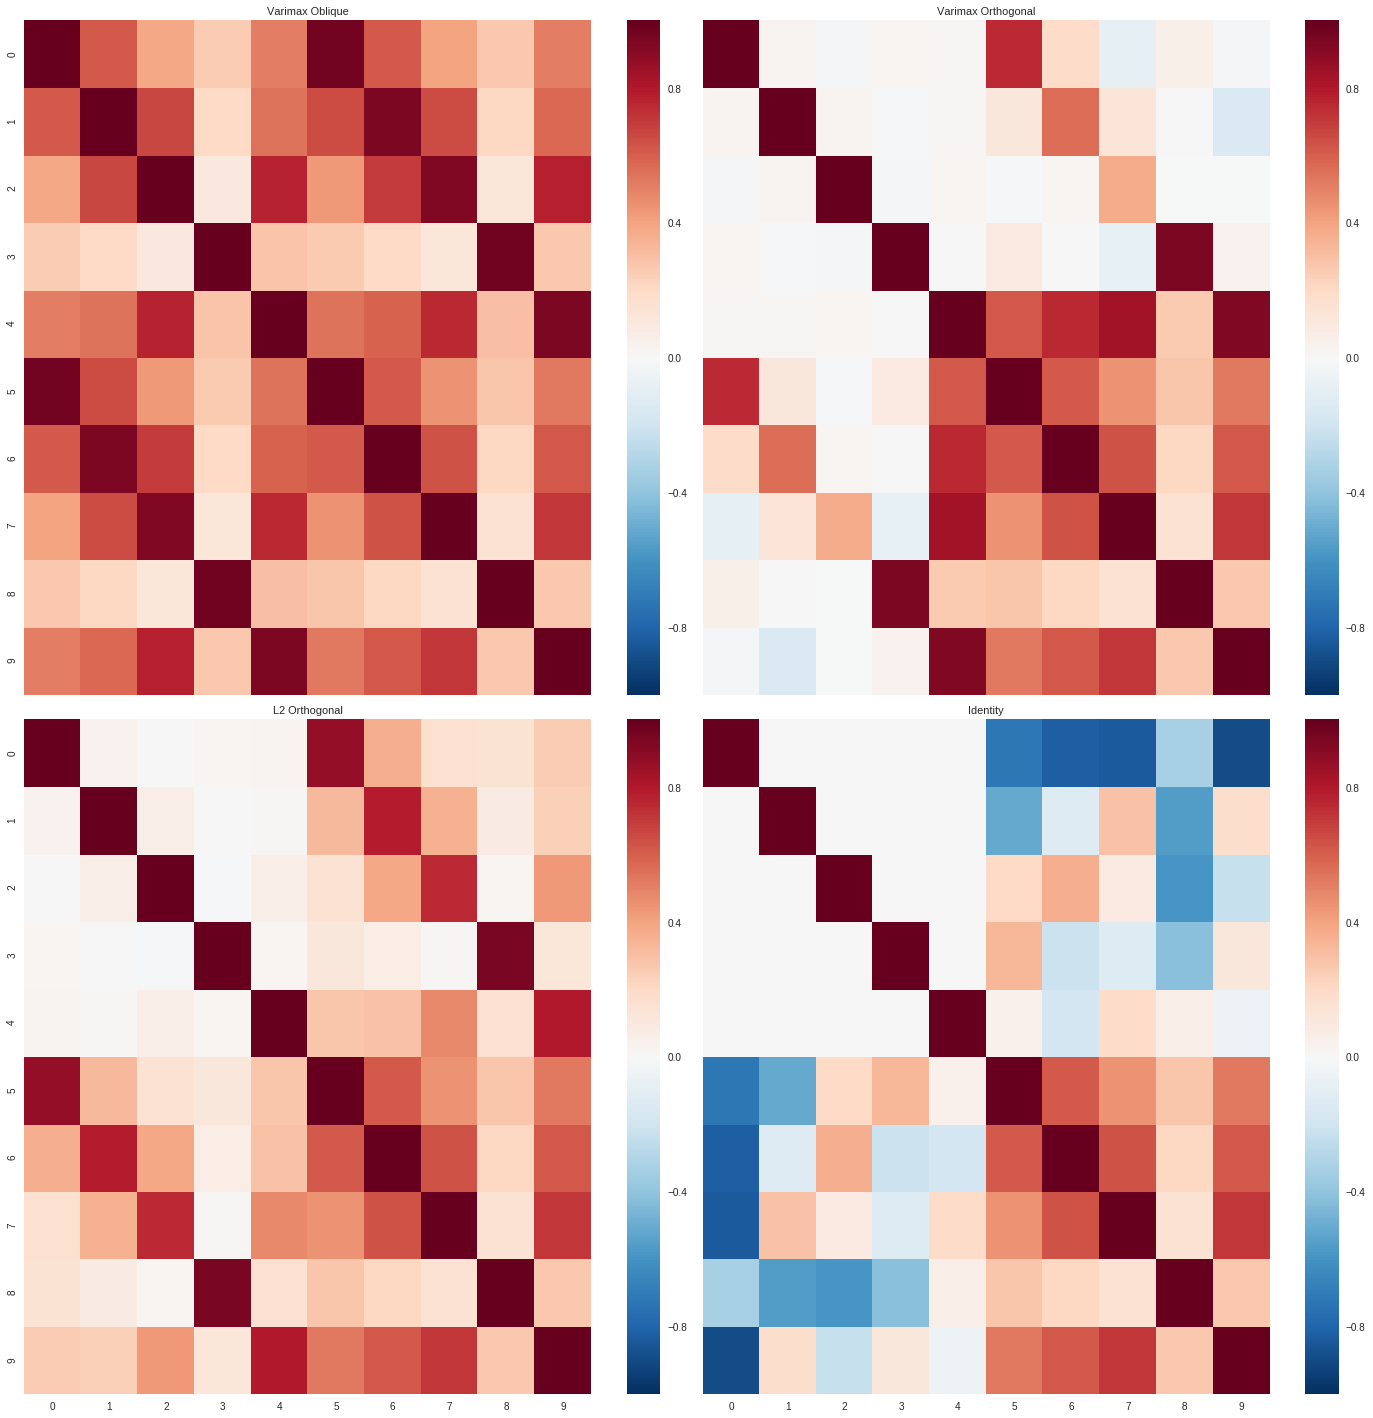
\includegraphics[width=\linewidth]{images/grid_bf.png}
\\
\\
\\
\begin{tabular}{lrrrrr}
\toprule
{} &         0 &         1 &         2 &         3 &         4 \\
\midrule
Varimax Oblique    &  0.968546 &  0.943092 &  0.922326 &  0.973424 &  0.942151 \\
Varimax Orthogonal &  0.748137 &  0.557080 &  0.369989 &  0.938690 &  0.932587 \\
L2 Orthogonal      &  0.881740 &  0.781647 &  0.747987 &  0.952970 &  0.802980 \\
Identity           &  0.331887 &  0.291065 &  0.359494 &  0.332125 &  0.195156 \\
\bottomrule
\end{tabular}
\caption{Different Rotations of Factors of Big Five Survey}\label{fig:grid-bf}
\end{figure}

\begin{figure}
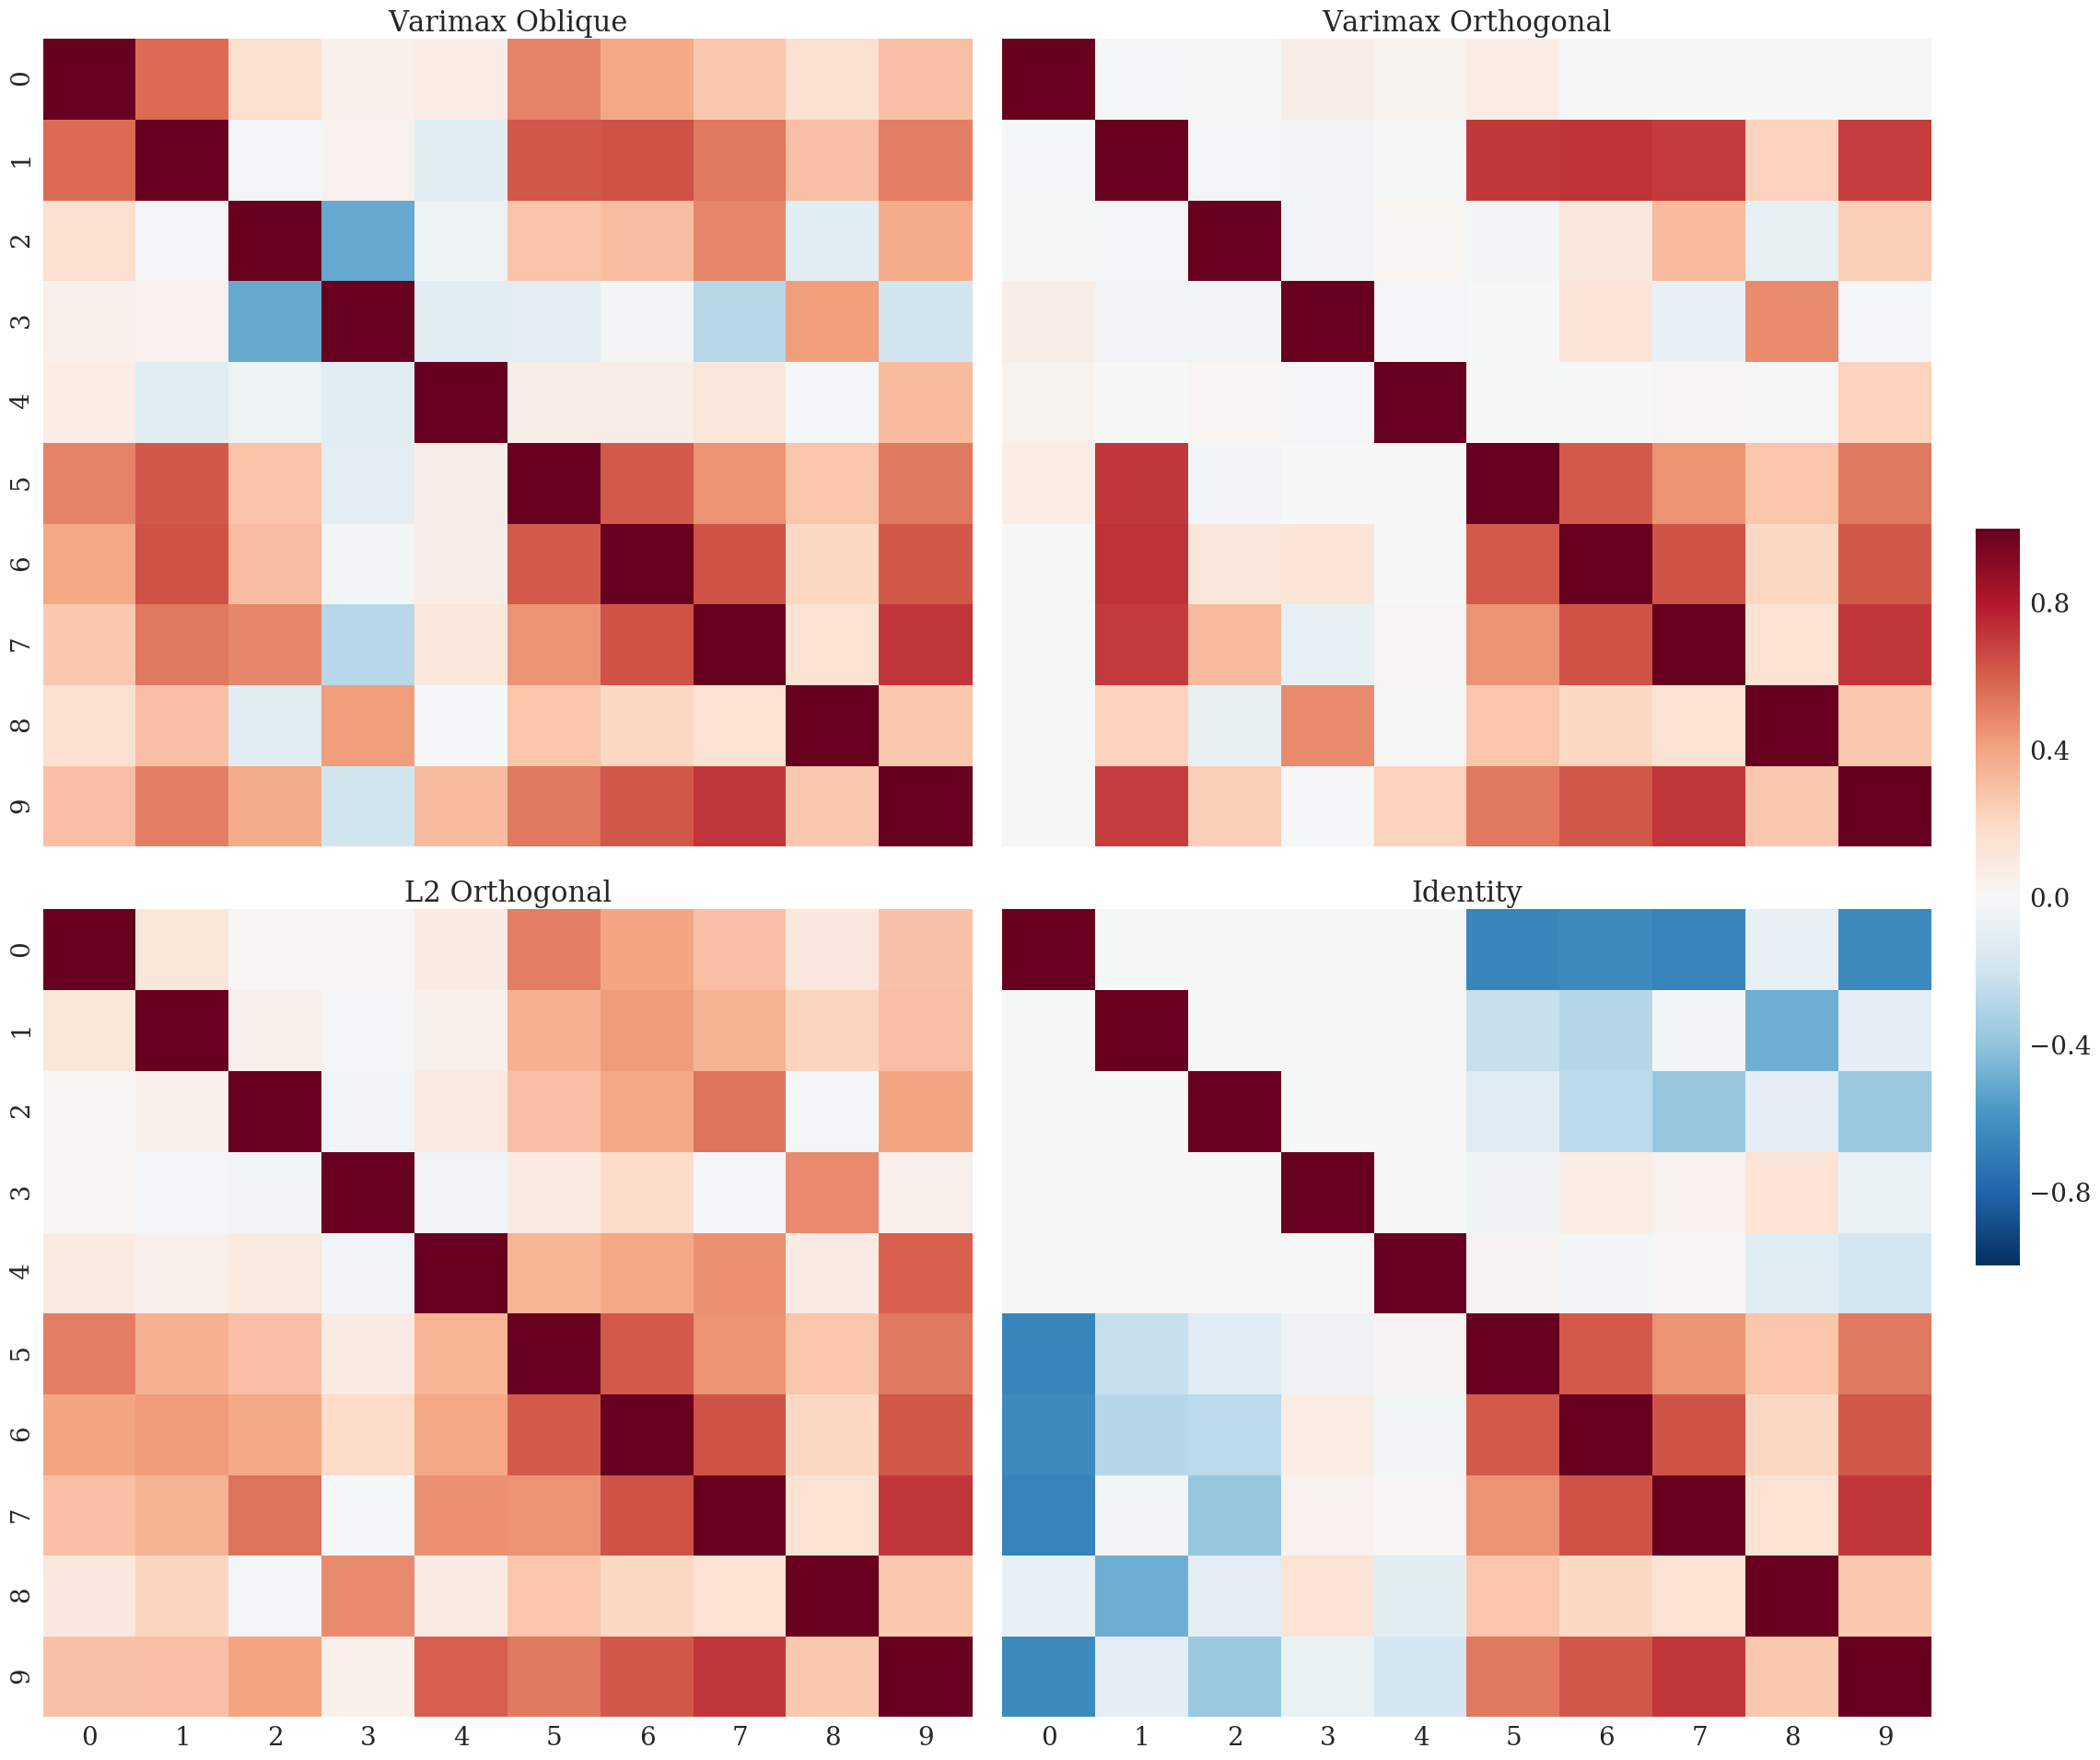
\includegraphics[width=\linewidth]{images/grid_others.png}
\\
\\
\\
\begin{tabular}{lrrrrr}
\toprule
{} &         0 &         1 &         2 &         3 &         4 \\
\midrule
Varimax Oblique    &  0.493596 &  0.639058 &  0.489409 &  0.421770 &  0.312784 \\
Varimax Orthogonal &  0.071356 &  0.725579 &  0.316222 &  0.470429 &  0.227975 \\
L2 Orthogonal      &  0.512753 &  0.423017 &  0.546490 &  0.469321 &  0.600568 \\
Identity           &  0.083879 &  0.025884 &  0.107176 &  0.134254 &  0.031207 \\
\bottomrule
\end{tabular}
\caption{Different Rotations of Factors of the Others Survey}\label{fig:grid-others}
\end{figure}


It can be clearly seen in the explained variance tables that the overall percentage of explained variance does not change with rotation, but that through varimax rotation the dispersion of variance is more equal, in line with the Big Five traits. This aligns with the previously stated theory, we are rotating the coordinate axes, but the subspace maintains the same, the rotation is done for our own purposes, in the traditional varimax case that purpose is to increase interpretability.

We hijack this process for our own purpose here, and explore several methods of rotating the coordinate axes such that we align the factors more closely with the big five, to see how well these factors might actually correlate with those of the Big Five, given the correct rotation.

To begin with we utilize a simple gradient projection algorithm, first introduced by Jennrich and summarized in \ref{2005gradient}, which is an optimization routine that allows us to rotate, both orthogonally and obliquely, by a given objective function for which gradients will be estimated numerically. We optimize three versions of this algorithm and plot correlation graphs between the rotated factors and the Big Five traits, one being the simple L2 norm difference between the matrices, the other being an oblique and orthogonal rotation of an objective function we create, which is simply the varimax of the correlation between the factors and the Big Five traits.

In this way we are taking this idea of simple structure and using it as a criterion for measuring how well our latent factors match the Big Five traits. Results of the correlation coefficients are plotted in figures \ref{fig:grid-bf} and \ref{fig:grid-others} and the maximum correlation with a Big Five factor is included for each factor. Note, that the factors are indexed 0-4, and the Big Five traits are indexed 5-10.

We take note of facts regarding the Big Five surveys and the Others survey:

\paragraph{Big Five Surveys}
While both the orthogonal L2 rotation and the orthogonal varimax rotation of the factors in the big five survey generate relatively high correlation coefficients with some of the Big Five traits, the oblique varimax iteration delivers scores that are extremely high, between 92-98\%. The success of all of the rotations leads us to a strong conclusion that these are the same latent factors, a major conclusion.

\paragraph{Others Survey}
Rotation of the factors in the Others survey, on the other hand, is decidedly less easy to interpret. The L2 approximation gives only three factors correlated more than 50\%, and the varimax, which has a simpler structure, only has one.
\\
\\
The natural next step, now that we're correlating latent factors, is to enter the world of Canonical Correspondence Analysis and Partial Least Square analysis, which attempts to do exactly that explicitly. There is a traditional algorithm, a few other versions, but for our purposes we explain the one that provides the best results in this circumstance, and happens to be so simple it can be accurately described in a catchphrase: PCA For Cross-Covariance Matrices. This is sometimes referred to as PLS-SVD, and it's brutally simply: we extract the SVD decomposition of the cross covariance matrix, and use the U and V as our loadings.

We rotate these orthogonally according to the L2 norm difference with Big Five traits, and see extremely promising results, with the highest correlation coefficients we've yet seen for the Other Surveys, with four of the factors with over 60\% correlation.

\begin{figure}
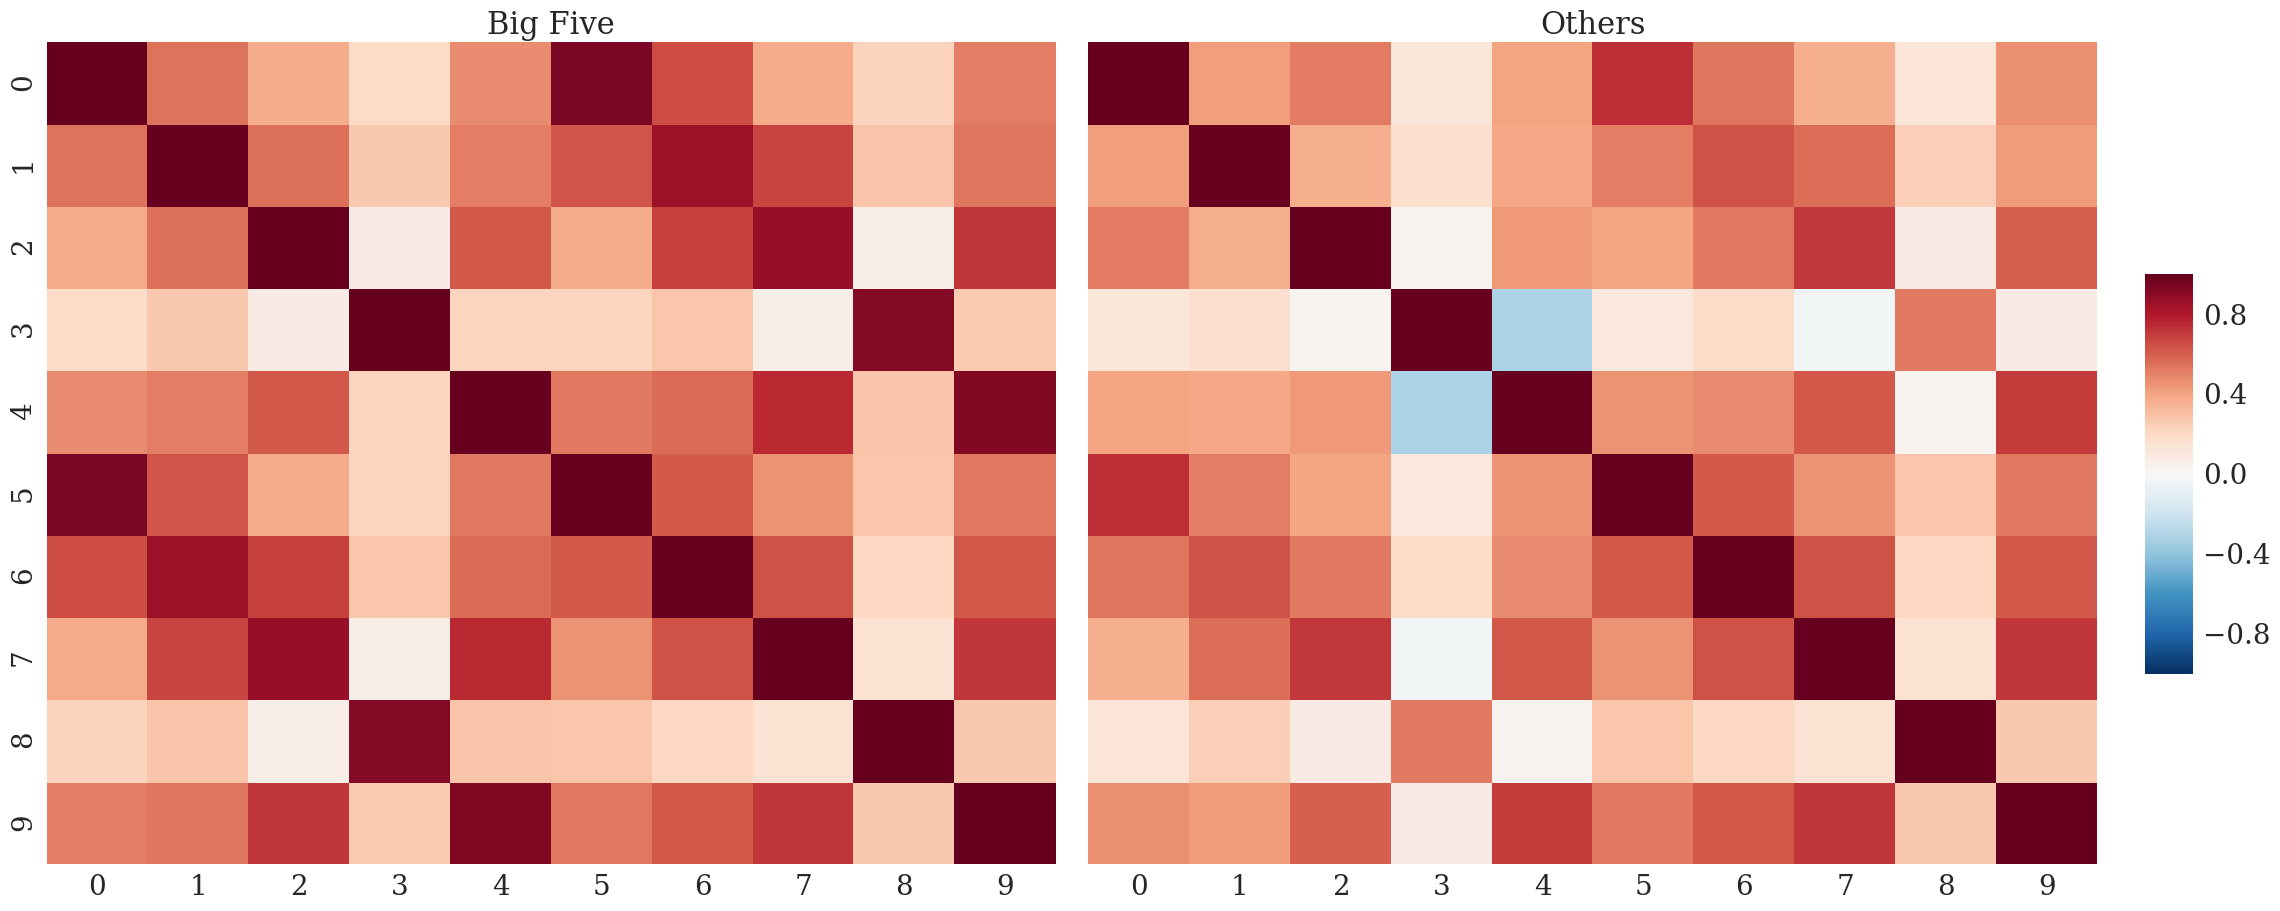
\includegraphics[width=\linewidth]{images/cross_svd.png}
\\
\\
\\
\begin{tabular}{lrrrrr}
\toprule
{} &         0 &         1 &         2 &         3 &         4 \\
\midrule
Big Five &  0.948249 &  0.858054 &  0.874393 &  0.915086 &  0.923285 \\
Others   &  0.741755 &  0.634072 &  0.703748 &  0.530984 &  0.696755 \\
\bottomrule
\end{tabular}
\caption{Correlation of L2 Rotated PLS-SVD}\label{fig:pls-svd}
\end{figure}


It is worth noting two interesting facts about all the above results that address directly the concern of Norman we recounted in the history section, namely: ``is there a large general factor, relating to general social desirability, present anywhere in these results.''

The first is the success of the oblique rotation, or the PLS-SVD which returned oblique factors. This is natural given the correlation of the Big Five traits in our data (lower left of the heat maps), but that in and of itself is concerning. Along with the way in which their is one trait that is completely uncorrelated with every other one (emotional instability), and combined with the single factor with extremely high variance in initial raw PCA and ML Factor Analysis runs, indicates that, quite possibly, there is one large general factor in our data. This is why allowing the first three factors to correlate produces higher coefficients.


\section{Regression}

A predictive model for multiple sources of high-dimensional data built on 94 observations on a cross-validated score alone is beyond the bounds of good conscious of this writer. As we have stated clearly in the beginning, we will need to rely on theory and decades of work in the field of personality psychology to make assumptions that allow us to accomplish this task, and the first of which is precisely the assumption we have attempted to validate in this thesis. The assumptions we will set in order to solve the prediction problem are:

\begin{enumerate}
\item The Big Five personality traits are alive and well in our population, and measurable through our data-collection techniques.

\item One or more of these traits will exist as important latent factors in every measurement we use to predict noncognitive skills of students.

\item For each measurement, the exact number or identification of exhibited traits is not determined ahead-of-time, but there will be prior beliefs.

\item Scoring will not necessarily be restricted to cardinal measures, in the realm of comparison and grading, ordinality will take precedence.
\end{enumerate}

Similarly, our ideal predictive model should relax the following assumptions which, while traditional to many instances of work in this field, will restrict us in flexibility to adopt the novel forms of data gathering and measurement that are core to the spirit of this work:

\begin{enumerate}
\item Gaussianity.
\item The linear relationship between latent factors and observed variables.
\end{enumerate}

We restrict postulations about the work or directions to find such a model to the conclusion. Instead, we will fit a linear regression model that fulfills none of the above requirements. We do this, naturally, as nothing more than an exercise, and include it out of interest.

For regression with a large number of highly correlated variables and an extremely small number of observations, we use elastic net regularization, whose parameters we pick via a grid search over 3-fold cross validation. The regularization of elastic net is given by:

$$
\hat{\beta} = \argmin_{\beta}||y - \mathbf{X}\beta ||^2 + \lambda_2|| \beta ||^2 + \lambda_1 || \beta ||_1
$$

This simple linear regression is surprisingly effective, we compare it to all other factor rotation techniques in a similar pattern as all our other plots, which can be seen in figure \ref{fig:regression}. We see that, with the exception of the problematic ``emotional instability'' trait from the Big Five, the factors of the linear regression have correlation coefficients over 80\% each. We cannot say that we have equal confidence as we did with the Big Five survey that the Big Five traits are the five major factors of the Other Surveys, but we have mounting evidence that there are at least three or four that may be present.

As mentioned in the outset, cardinality as a measure of cost for our factor estimation is not useful for our context, and this regression was run with a standard squared cardinal loss function, and we refrain from examining further characteristics of this result as, as previously emphasized, it is included for comparison to the factor rotation techniques, to provide a context for them.

We note that again we see that the factors found by the regression are highly correlated, except for the single outlying ``emotional instability.''



\begin{figure}
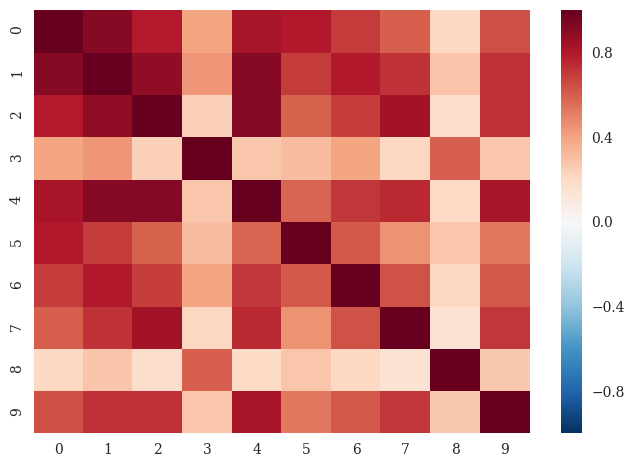
\includegraphics[width=\linewidth]{images/linear_reg.png}
\\
\\
\\
\begin{tabular}{lrrrrr}
\toprule
{} &         0 &         1 &         2 &         3 &         4 \\
\midrule
Linear Regression &  0.800271 &  0.803592 &  0.840472 &  0.599498 &  0.825383 \\
\bottomrule
\end{tabular}
\caption{Correlation of Factors Found by Linear Regression}\label{fig:regression}
\end{figure}

\section{Conclusion}

We have unearthed the original techniques, theories, and concerns of the original authors of the Big Five personality traits and determined resoundingly that, indeed, these traits are present and measurable in the population and data-collection methods we are using in our work. Specifically, we found that each of the five major factors self-evident in the data of the Big Five survey are extremely correlated with each of the Big Five personality traits.

The results for the Other surveys are quite mixed, where at most three or possibly four of the driving factors from that space can be identified to Big Five traits.

We raised a serious concern about the existence of a single general factor, which combined with the asymmetric answers to some of the survey questions could indicate that the surveys themselves are misaligned with the population. This was a confounding factor in our ability to determine the Big Five traits, and while it was not in the end insurmountable, it is definite cause for concern and caution in future efforts.

This was the primary purpose of this thesis, however, as is so often the case, we have opened more questions than we have closed and much work is still to be done.

The clearest work that lays ahead is to begin the process of building a predictive model that incorporates all of the assumptions laid out in the Regression section. All of our assumptions beg us to consider the world of Bayesian Non-Parametric modeling, which give us both formal Bayesian formulations of prior belief, flexibility with regards to distributions of errors and linearlity of relationships, as well as the ability to avoid setting the number of parameters, in our case latent factors to be learned, a prior. There has been relatively little work in this relatively recent field, with notable exceptions being \cite{}.



\printbibliography
\end{document}